\documentclass{article}[18pt]
\usepackage{../../../../format}
\lhead{Software Engineering - Software Design}


\begin{document}
\begin{center}
\underline{\huge The major forms of architectural style}
\end{center}
\section{Call and return}
Characterised by:
\begin{itemize}
	\item Order of computation (sequencing of control)
	\item Only a single thread of control (no concurrency)
	\item Structures organised around computational tasks
\end{itemize}
Type of reasoning:
\begin{itemize}
	\item Hierarchical, organised around control being passed from "higher" to "lower" items
	\item Task performed by a set of sub-tasks
	\item Explicit control linkages between the subtasks and the algorithm of the program to determine calling order
\end{itemize}
\subsection{Example 1}
Main program/sub-programs:
\begin{itemize}
	\item Components are subprograms
	\item Connectors are the invocation links (including parameters)
\end{itemize}
This is the form that is embodied in most non-OO imperative programming languages
\begin{center}
	\includegraphics[scale=0.7]{"Call and Return"}
\end{center}
\subsection{Example 2}
Classical objects - here the methods are part of the objects:
\begin{itemize}
	\item Components are both the objects and also their methods/data
	\item Connectors are the method calls and parameters
\end{itemize}
Supported by object-based and object-oriented programming languages. May use run-time bindings
\begin{center}
	\includegraphics[scale=0.7]{"Call and Return1"}
\end{center}
\section{Interacting Processes}
Characterised by:
\begin{itemize}
	\item Communication patterns among independent, usually concurrent, processes
	\item Independent elements can be objects, lightweight processes, services etc
	\item Context is more complex as emphasis is upon "interaction"
\end{itemize}
Type of reasoning
\begin{itemize}
	\item Non-deterministic - scheduling of system elements is performed by separate, independent computers
	\item Design based around these independent actions and needs to specifically address any requirements that impose the need for particular sequences or interactions
\end{itemize}
\subsection{Communicating processes}
Based around a network of processes running on different machines and linked via Remote Procedure Calls (RPC)
\begin{itemize}
	\item Components are the processes
	\item Connectors are the message protocols via RPCs
\end{itemize}
Binding time can be at each construction or when the system is started. Each system runs in its own address space - no direct access to shared data
\begin{center}
	\includegraphics[scale=0.7]{"Communicating Processes"}
\end{center}
\subsection{Lightweight processes (threads)}
A thread is a block of code that can be executed independently of other threads within the program
\begin{itemize}
	\item Components are the threads
	\item Connectors are provided largely by using shared data
\end{itemize}
Because threads are part of a single process, they have a shared data space, needing care with synchronisation of access
\begin{center}
	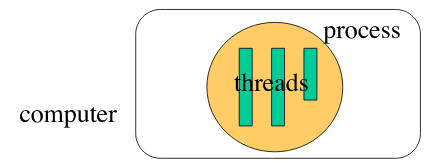
\includegraphics[scale=0.7]{Threads}
\end{center}
\section{Data-Centred Repository}
Characterised by:
\begin{itemize}
	\item A dominant central data store that is manipulated by independent communications
	\item Centred around the issues relating to data access 
	\item Data is at the focus
\end{itemize}
Type of reasoning:
\begin{itemize}
	\item Can depend on the form of the system
	\item For databases it is the ACID properties
	\item Includes modern compilers
\end{itemize}
\subsection{Transactional Database}
The classical idea of the data-centred repository
\begin{itemize}
	\item Components - Memory and computations within the database
	\item Connectors - Transaction streams (queries)
\end{itemize}
Style is not concerned with the internal form of the database, only with its role
\begin{center}
	\includegraphics[scale=0.7]{"Transactional Database"}
\end{center}
\subsection{Client-Server}
A "distributed" form using a "thin" client process to interact with the end-users. While the server often incorporates a database, this is not a necessity
\begin{itemize}
	\item Components - Data managers and computations
	\item Connectors - Transaction operations with history
\end{itemize}







\end{document}